\documentclass[11pt,a4paper]{article}

\usepackage[colorlinks=true, linkcolor=black!50!blue, urlcolor=blue, citecolor=blue, anchorcolor=blue]{hyperref}
\usepackage[font=small,labelfont=bf,margin=0mm,labelsep=period,tableposition=top]{caption}
\usepackage[a4paper,top=3cm,bottom=2.5cm,left=2.5cm,right=2.5cm,bindingoffset=0mm]{geometry}

\usepackage{graphicx}
\usepackage{float}
\usepackage{afterpage}
\usepackage{epsfig,cite}
\usepackage{amssymb}
\usepackage{amsmath}
\usepackage{bm}
\usepackage{dsfont}
\usepackage{multirow}
\usepackage{url}
\usepackage{xcolor}
\usepackage{float}
\usepackage{afterpage}
\usepackage{ulem}

\usepackage{url}
\usepackage{hyperref}

\usepackage{multirow,booktabs,multirow}

\bibliographystyle{JHEP}

%%%%%%%%%%%%%%%%%%%%%%%%%%%%%%%%%%%%%%%%%%%%%%%%%%%%%%%%%%%%%

\def\smallfrac#1#2{\hbox{$\frac{#1}{#2}$}}
\newcommand{\be}{\begin{equation}}
\newcommand{\ee}{\end{equation}}
\newcommand{\bea}{\begin{eqnarray}}
\newcommand{\eea}{\end{eqnarray}}
\newcommand{\bi}{\begin{itemize}}
\newcommand{\ei}{\end{itemize}}
\newcommand{\ben}{\begin{enumerate}}
\newcommand{\een}{\end{enumerate}}
\newcommand{\la}{\left\langle}
\newcommand{\ra}{\right\rangle}
\newcommand{\lc}{\left[}
\newcommand{\rc}{\right]}
\newcommand{\lp}{\left(}
\newcommand{\rp}{\right)}
\newcommand{\as}{\alpha_s}
\newcommand{\aq}{\alpha_s\left( Q^2 \right)}
\newcommand{\amz}{\alpha_s\left( M_Z^2 \right)}
\newcommand{\aqq}{\alpha_s \left( Q^2_0 \right)}
\newcommand{\aqz}{\alpha_s \left( Q^2_0 \right)}
\def\toinf#1{\mathrel{\mathop{\sim}\limits_{\scriptscriptstyle
{#1\rightarrow\infty }}}}
\def\tozero#1{\mathrel{\mathop{\sim}\limits_{\scriptscriptstyle
{#1\rightarrow0 }}}}
\def\toone#1{\mathrel{\mathop{\sim}\limits_{\scriptscriptstyle
{#1\rightarrow1 }}}}
\def\frac#1#2{{{#1}\over {#2}}}
\def\gsim{\mathrel{\rlap{\lower4pt\hbox{\hskip1pt$\sim$}}
    \raise1pt\hbox{$>$}}}       
\def\lsim{\mathrel{\rlap{\lower4pt\hbox{\hskip1pt$\sim$}}
    \raise1pt\hbox{$<$}}}       
\newcommand{\mrexp}{\mathrm{exp}}
\newcommand{\dat}{\mathrm{dat}}
\newcommand{\one}{\mathrm{(1)}}
\newcommand{\two}{\mathrm{(2)}}
\newcommand{\art}{\mathrm{art}}
\newcommand{\rep}{\mathrm{rep}}
\newcommand{\net}{\mathrm{net}}
\newcommand{\stopp}{\mathrm{stop}}
\newcommand{\sys}{\mathrm{sys}}
\newcommand{\stat}{\mathrm{stat}}
\newcommand{\diag}{\mathrm{diag}}
\newcommand{\pdf}{\mathrm{pdf}}
\newcommand{\tot}{\mathrm{tot}}
\newcommand{\minn}{\mathrm{min}}
\newcommand{\mut}{\mathrm{mut}}
\newcommand{\partt}{\mathrm{part}}
\newcommand{\dof}{\mathrm{dof}}
\newcommand{\NS}{\mathrm{NS}}
\newcommand{\cov}{\mathrm{cov}}
\newcommand{\gen}{\mathrm{gen}}
\newcommand{\cut}{\mathrm{cut}}
\newcommand{\parr}{\mathrm{par}}
\newcommand{\val}{\mathrm{val}}
\newcommand{\tr}{\mathrm{tr}}
\newcommand{\checkk}{\mathrm{check}}
\newcommand{\reff}{\mathrm{ref}}
\newcommand{\Mll}{M_{ll}}
\newcommand{\extra}{\mathrm{extra}}
\newcommand{\draft}[1]{}
\newcommand{\comment}[1]{{\bf \it  #1}}
\def\beq{\begin{equation}}
\def\eeq{\end{equation}}

% Added by MU 
\def \a{\alpha}
\def \b{\beta}
\def \g{\gamma}
\def \z{\zeta}
\def \t{{\bf T}} % vector of theoretical predictions
\def \c{{\bf c}} % vector of coefficients of theoretical predictions
\def \y{{\bf y}} % vector of experimental data
\def \s{{\bf \sigma}} % experimental covariance matrix
% Added by JR
\def\lapprox{\lower .7ex\hbox{$\;\stackrel{\textstyle <}{\sim}\;$}}
\def\gapprox{\lower .7ex\hbox{$\;\stackrel{\textstyle >}{\sim}\;$}}
\def\half{\smallfrac{1}{2}}
\def\GeV{{\rm GeV}}
\def\TeV{{\rm TeV}}
\def\ap{{a'}}
\def\vp{{v'}}
\def\e{\epsilon}
\def\d{{\rm d}}
\def\calN{{\cal N}}
\def\shat{\hat{s}}
\def\barq{\bar{q}}
\def\qq{q \bar q}
\def\uu{u \bar u}
\def\dd{d \bar d}
\def\pp{p \bar p}
\def\xa{x_{1}}
\def\xb{x_{2}}
\def\xaa{x_{1}^{0}}
\def\xbb{x_{2}^{0}}
\def\smx{\stackrel{x\to 0}{\longrightarrow}}
\def\Li{{\rm Li}}

\numberwithin{equation}{section}
\numberwithin{figure}{section}
\numberwithin{table}{section}

\newcommand{\tmop}[1]{\ensuremath{\operatorname{#1}}}
\newcommand{\tmtextit}[1]{{\itshape{#1}}}
\newcommand{\tmtextrm}[1]{{\rmfamily{#1}}}
\newcommand{\tmtexttt}[1]{{\ttfamily{#1}}}

\usepackage{tabularx}
\newcolumntype{C}[1]{>{\centering\arraybackslash}p{#1}}

\begin{document}
\newgeometry{top=1.5cm,bottom=1.5cm,left=2.5cm,right=2.5cm,bindingoffset=0mm}

\vspace{2cm}

\begin{center}
  {\Large \bf
  Accessing the low-loss region in EELS with machine learning
  }
\vspace{1.4cm}


 Laurien, Luigi, Juan and Sonia\\


\vspace{0.4cm}
       {\it TU Delft and Nikhef
       }

       \vspace{1.0cm}

       {\bf \large Abstract}
       
\end{center}

We use neural networks and Monte Carlo sampling techniques
to provide a model-independent determination of the zero-loss peak
in electron energy-loss spectroscopy (EELS) measurements with faithful uncertainty estimation.

\tableofcontents

\section{Introduction}

Intro to the general problem of low-loss EELS and ZLP background subtraction.

Motivation of the specific materials.

Motivation for the HEP techniques in the context of material sciences.

In this work we will follow the approach pioneering by the NNPDF collaboration~\cite{Ball:2017nwa}.

\section{Data samples}

The spectra used for the purpose of this study are retrieved from the studies of Miguel Tinoco, Luigi Maduro et. al.  \cite{soniamos2} on specific structures of molybdenum disulfide (MoS2). MoS2 is a highly promising material exhibiting a wide range of possible applications for electronic and optical devices. When MoS2 is thinned down to a single monolayer (ML), its indirect band gap switches to a direct band gap of around 1.88 eV \cite{nerl}. \\
A monochromated electron source was used operating at 60 kV, which achieves an energy resolution of around 30 meV. The most-distinctive features of the EELS spectra are two relatively narrow peaks around 1.88 and 2.05 eV, arising from the direct exciton transitions and split by interlayer interactions and spin-orbit coupling. These measurements for the position of the bandgap is consistent with previous studies \cite{nerl, komsa}. The peaks could be revealed after subtraction of a fitted Gaussian curve and a power law to the ZLP and its right-hand tail. \\

An ensemble of electron loss spectra acquired at different positions at the sample is used to construct the training inputs (Fig. \ref{spectra}). As the ZLP is several orders of magnitude bigger than the sample data, the logarithm of the intensity is used to train the model.

\begin{figure}[H]
    \centering
    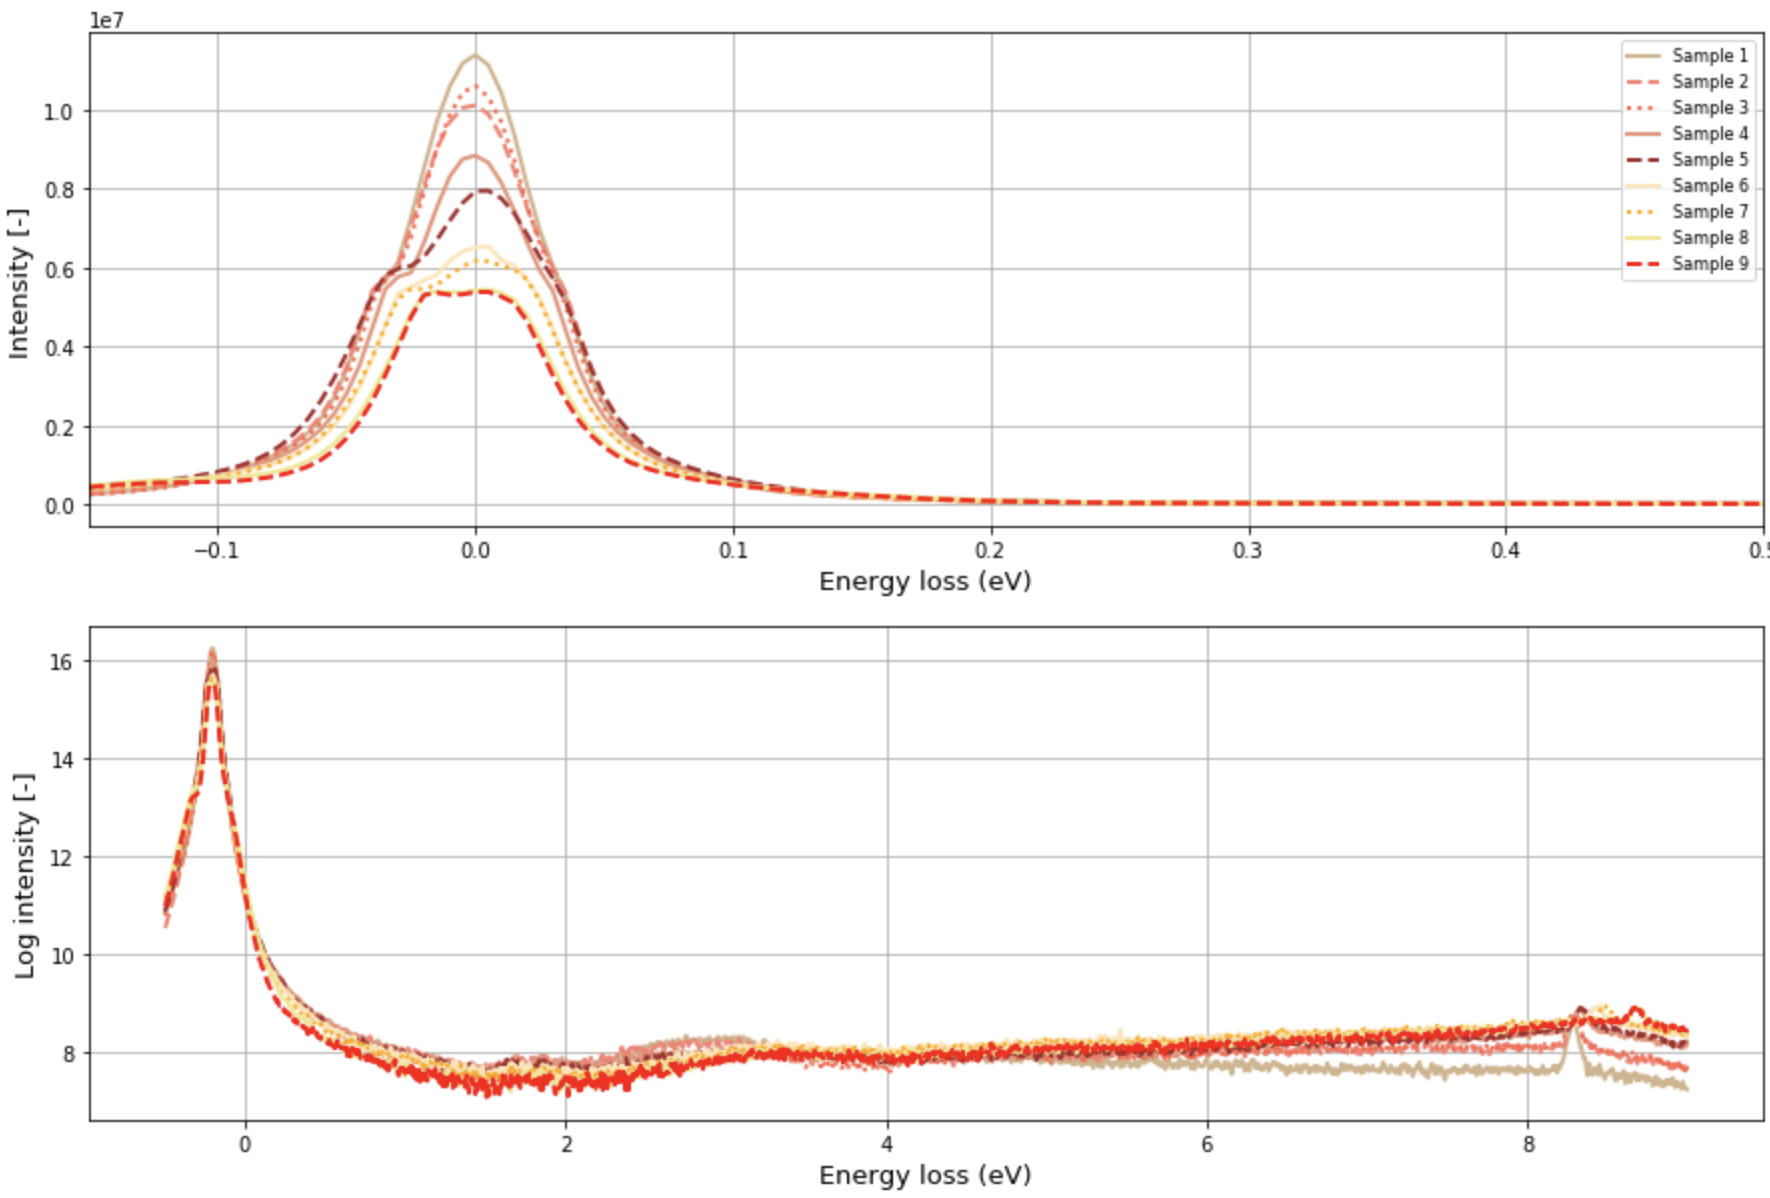
\includegraphics[width=130mm]{plots/spectrum.png}
    \caption{Energy electron loss spectra taken at nine different positions on a sample of MoS2. Up: original intensity. Below: logarithmic intensity. Retrieved from \cite{soniamos2}. }
    \label{spectra}
\end{figure}


\section{Methodology}

\subsection{Preprocessing}
Unscaled input variables can result in a slow or unstable learning process, whereas unscaled target variables on regression problems can result in exploding gradients causing the learning process to fail \cite{juan}. The energy loss is scaled between [$-1,1$] and all input spectra are scaled between [$0.1, 0.9$]. \\

The discretization technique used to assign mean and standard deviation the data points is Equal Width Discretization (EWD) \cite{ewd}. EWD is a simple discretization method that divides the range of observed values for a feature into k equal sized bins. The intervals are computed by 
 $\Delta E = (E_{max} - E_{min}) / k$. The value of k is chosen empirically such that the number of bins is high enough to not lose valuable information, but still contains a sufficient number of data points to calculate the uncertainties.\
Within each energy bin $\Delta E$, the median and variance of all data points within this bin are determined and returned to the original data points. This way, each data point is a vector $[dE, D_i, \sigma_i]$ where dE is the original energy loss; $D_i$ and $\sigma_i$ are the median and std of the bin $i$ where this point belongs to. 
The energy loss of the sample data covers a $[-0.3, 8]$ eV range. Since the ZLP feature is several orders of magnitude bigger than the sample features, we take the logarithm of the intensity to train the network. 
\\

\begin{figure}[H]
    \centering
    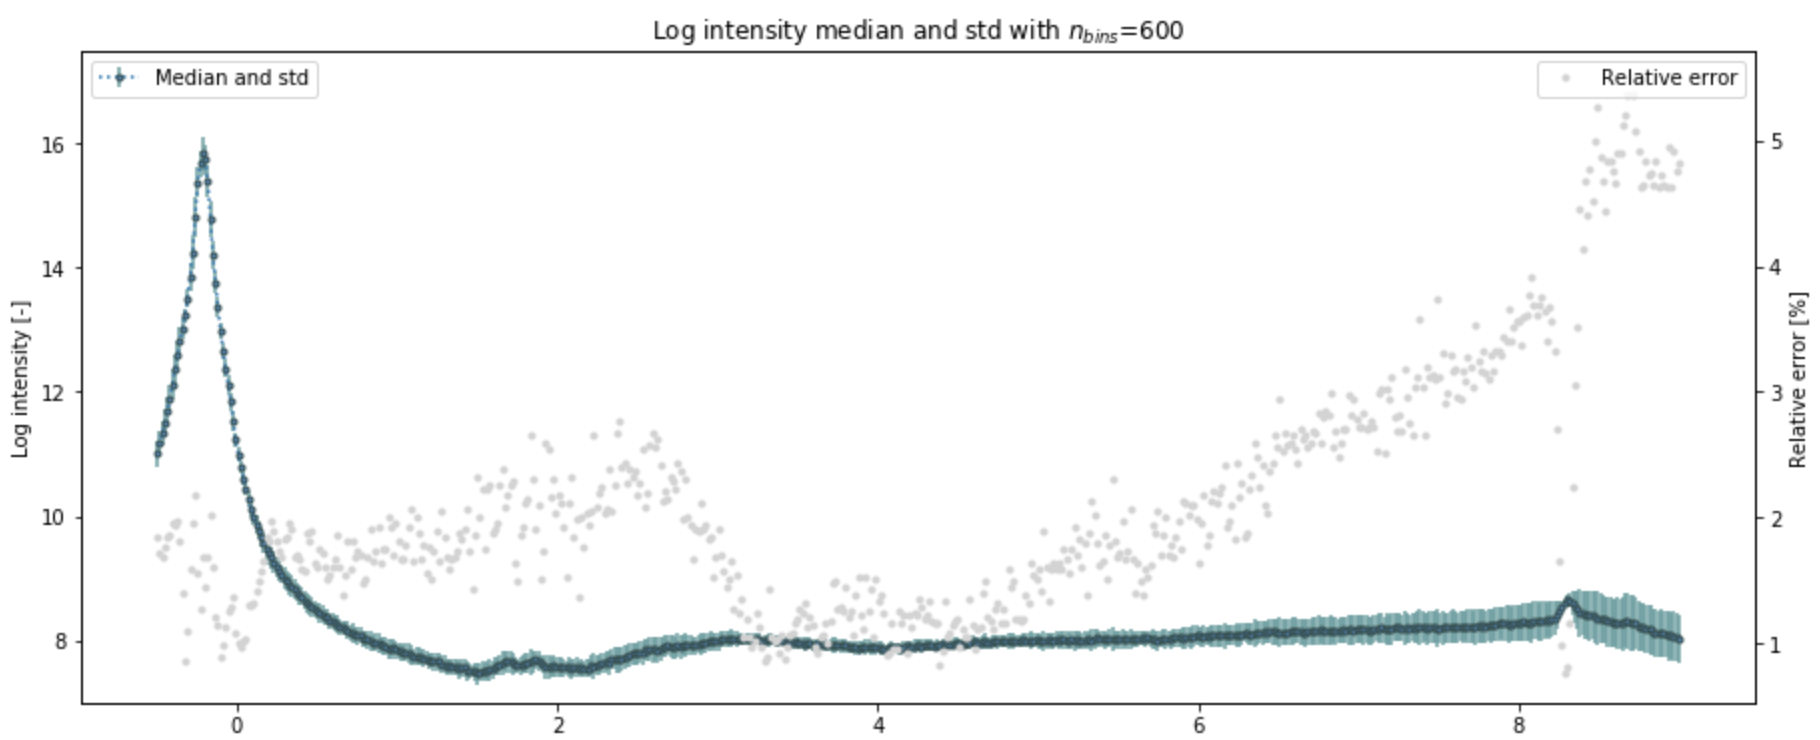
\includegraphics[width=155mm]{plots/ewd.png}
    \caption{Log intensity profile of the sample data after applying EWD with $n_{bins}$=600.}
    \label{ranges}
\end{figure}

\subsubsection{Closure Testing}
In order to validate if the computed error associated to each training point is reasonable, a method called Closure Testing provides insight \cite{closure}.  The 'true' values are then the best Gaussian fit sampled at the energy data of the training points. Sampling this Gaussian at the points $(dE_i)$ where we have data and fluctuating it by a Gaussian random number with size $\sigma_i$ returns a $\chi^2$ of 1, indicating that the computed errors by means of EWD are a good approximation.\\



\subsection{Training regions}
It is important to make an informed choice as to the energy range of the input data over which the neural network is trained. Figure \ref{ranges} below is a schematic low-loss spectrum showing five relevant energy ranges \cite{reed}. Region (a) doesn't contain loss electrons and contributions solely come from dark counts in the detector. Range (b) and (c) together form the 'ZLP-region', with the left- and right hand side of the ZLP respectively. Since we make use of a monochromated electron beam, the energy distribution is approximately symmetric around zero and range (c) will be the mirrored version of range (b) until a certain energy limit, which we will call $dE_1$. Range (e) sets in at higher energy loss $dE_2$ and represents the almost pure loss signal, with essentially negligible ZLP contributions. Region (d) is the transition in which the ZLP tail gradually gives way to the loss signal. It is this region that is specifically of interest, as it contains the low-loss features of the sample.  Our objective is to automatically determine the right values for $dE_1$ and $dE_2$ before training the neural network.

\begin{figure}[H]
    \centering
    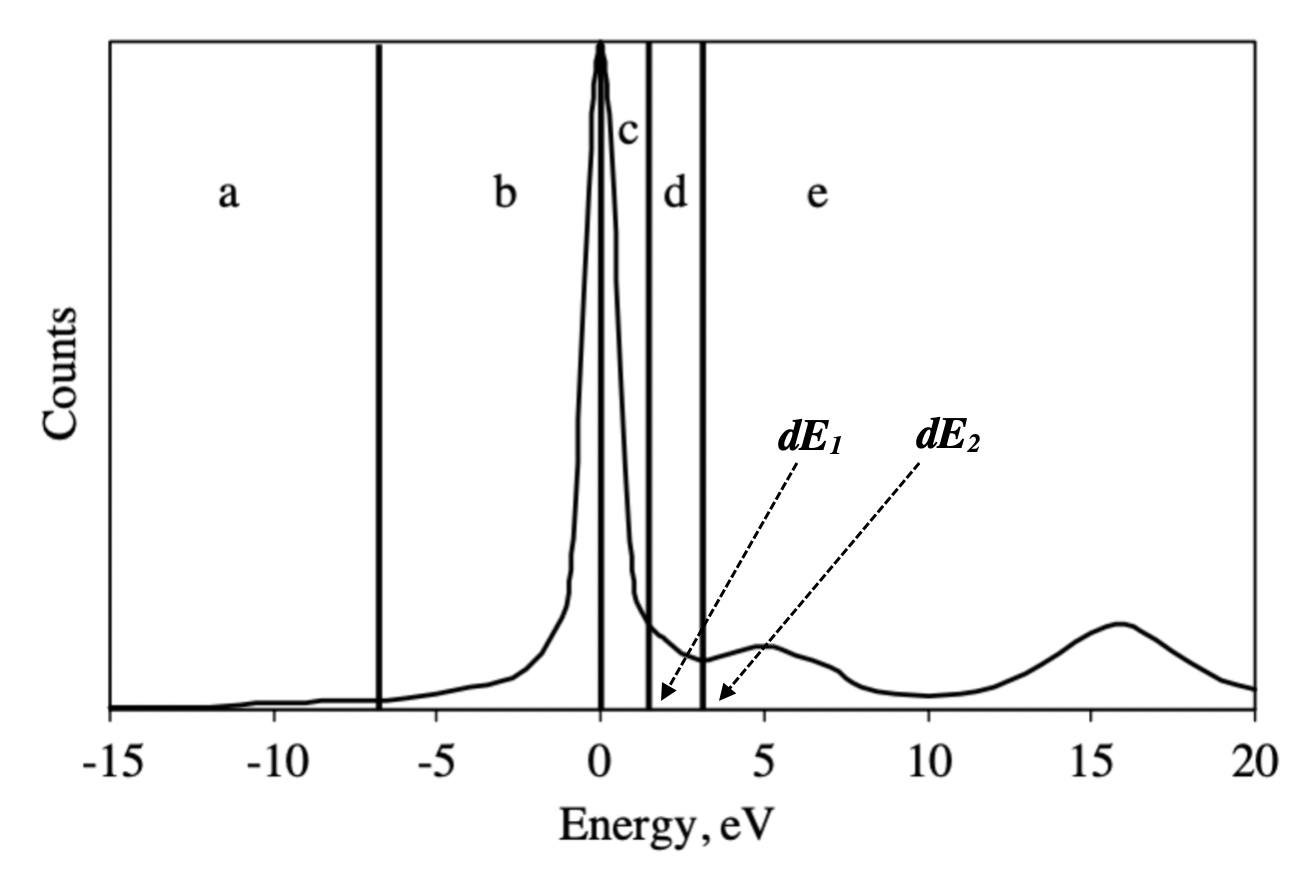
\includegraphics[width=100mm]{plots/ranges.png}
    \caption{Schematic illustration of the relevant energy ranges used in the model}
    \label{ranges}
\end{figure}

Before training, a window is to be applied to the training inputs to an upper boundary $dE_1$, to ensure the network trains on data of the ZLP solely. In order to attain a model that meets $log(I_{ZLP}) \rightarrow 0$ as $dE \rightarrow \infty$, pseudo data is to be added for $E>dE_2$ where the ZLP contribution becomes negligible. The model is trained on data for $E<dE_1$ and $E>dE_2$, the interpolation region $dE_1 < E < dE_2$ contains the predictions of interest. \\

In order to set the right values for $dE_1$ and $dE_2$, we look at the ratio 
\begin{equation}
    R = \frac{I(sample)}{I(ZLP)}
\end{equation}
at any point over the spectrum, where $I(sample)$ and $I(ZLP)$ are the intensity of the sample and the reference ZLP respectively. This way it is convenient to define three regions: the 'ZLP region' where $R\ll1$, corresponding to region (a)-(c) ending at , the 'transition region' (d) starting at $dE_1$ and ending at $dE_2$, and the 'sample region' (e) with $R\gg1$.\\

In an ideal microscope the electron beam would be perfectly monochromatic, correspondingly the ZLP would appear as a delta function in an EEL spectrum \cite{rafferty}. In practice the ZLP has a finite width defining the energy resolution of the system. At some energy loss the contribution to the sample kicks in, rapidly increasing the value of $R$. It is at this point that the intensity profile, earlier monotonically decreasing, will have its first local minimum and correspondingly the first derivative will cross zero. By calculating the log derivative of the mean sample intensity, we can conclude that  $\frac{d}{dE}log(I)=0$ at $dE_2$ = $1.715$ eV  (Fig. \ref{bound}). 

\begin{figure}[H]
    \centering 
    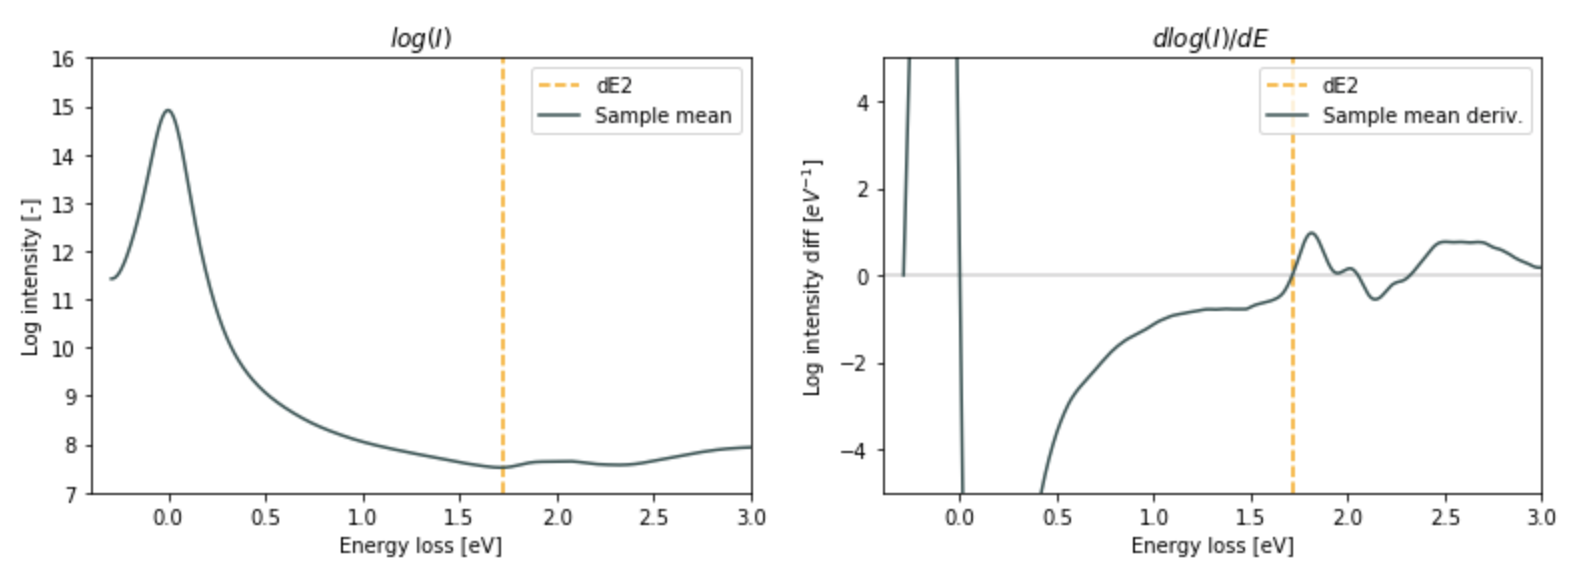
\includegraphics[width=150mm]{plots/bound.png}
    \caption{Log and log derivative of the sample intensity. The intensity profile is calculated as the median over the collection of training samples. The crossing of the first derivative with zero is \textbf{1.715} eV and marks the transition to the sample region ($dE_2$). Before taking the derivative, smoothing by means of a Hann window \cite{hann} was applied to log(I) to remove noise and reveal underlying trends. }
    \label{bound}
\end{figure}

By stating that the ideal zero loss peak is symmetric around zero up to energy loss $dE_1$, hypothetically we could determine its value by mirroring the left-hand tail to the right side and see when the two significantly start to deviate. In practice however, the ZLP is not symmetric due to various external factors such as astigmatism \cite{astigma} and virtual scattering events \cite{rafferty}, which makes direct reflection of the left-hand tail unfavorable. \\
The value of $dE_1$ will be chosen as $dE_2 / a$, with $a$ a positive integer. The choice of $a$ is empirical and will be cross-validated. \\ \newpage

After the choice on $dE_1$ and $dE_2$, the set of training data (TD) will be prepared taking the following steps:
\begin{enumerate}
    \item Keep only sample data (SD) inside the window [$dE_{min}, dE_1$]
    \item Create pseudo data (PD) with $log(I)$=0 in range [$dE_2, dE_{max}$]
    \item TD = SD + PD
\end{enumerate}

\subsection{Monte Carlo sampling}
Training points are generated by Monte Carlo sampling; for the set of training points $[dE, D_i, \sigma_i]$, a set of MC training points is generated by adding a stochastic noise signal on top of the the data with a std equal to the corresponding error on that point. 

\begin{itemize}
    \item $train_x$: dE
    \item $train_y$: $D_i$ + rand.norm(0, $\sigma_i$)
\end{itemize}

Repetitive training of the NN (number of repetitions = $N_{rep}$) on each set of MC pseudo data yields a prediction that is distributed with a mean and std corresponding to the mean and error of the original training set. \\
... to be continued

\section{Results}
Here we present the main results of this paper

\section{Summary and outlook}
....

\bibliography{main}
\end{document}

